\documentclass[11pt,a4paper]{article}
\usepackage[margin=23mm,headheight=15pt]{geometry}
\usepackage[T1]{fontenc}\usepackage{tgpagella}\usepackage{amsmath,amssymb,mathtools,bm,booktabs,longtable,array,microtype,xcolor,tikz,fancyhdr,hyperref,enumitem}
\usetikzlibrary{arrows.meta,decorations.pathmorphing,positioning,calc}
\hypersetup{colorlinks=true,linkcolor=blue!55!black,urlcolor=blue!55!black}
\definecolor{ink}{RGB}{24,40,68}\definecolor{violet}{RGB}{105,64,172}
\pagestyle{fancy}\fancyhf{}\fancyhead[L]{\small Quantum Atomic Physics Companion}\fancyhead[R]{\small Chapter III --- Optical Lattices}\fancyfoot[C]{\thepage}
\setlength{\parskip}{5pt}\setlength{\parindent}{0pt}
\newcommand{\ex}[1]{\subsection*{Worked Example #1}}
\newcommand{\ee}{\mathrm E}
\usepackage{amsthm}
\newtheorem{example}{Worked Example}
\begin{document}
\begin{center}
{\LARGE\bfseries\color{ink} Quantum Gases in Optical Lattices}\\[5pt]
{\Large From Rubidium Condensates to the Bose--Hubbard Model}\\[8pt]
{\small Advanced Quantum Physics Companion --- Chapter III}\end{center}
\begin{abstract}
This chapter continues the distinction between bound electronic orbitals of neutral rubidium and external motional orbitals of whole atoms. We derive optical-lattice potentials, recoil scales, Bloch and Wannier states, and the Bose--Hubbard Hamiltonian. Ten detailed worked examples connect tunneling, interactions, coherent and Mott states, number fluctuations and time-of-flight interference. Throughout, a lattice of trapped atoms is distinguished from an electronic crystal and the picokelvin Tiangong free-expansion experiment.
\end{abstract}
\tableofcontents\newpage
\section{Three systems that must not be confused}
A neutral $^{87}\mathrm{Rb}$ atom contains 37 protons, 50 neutrons and 37 electrons. The valence electron is in the ground electronic configuration $[\mathrm{Kr}]5s^1$. Its $5s$ orbital is an \emph{internal electronic} orbital. A whole atom in a trap has an independent \emph{center-of-mass} orbital. In a quantum-degenerate gas many identical bosonic atoms can macroscopically occupy a common motional state. In an optical lattice, the motional state is modified by a periodic external potential; no periodic chemical array of rubidium ions is required.
\begin{center}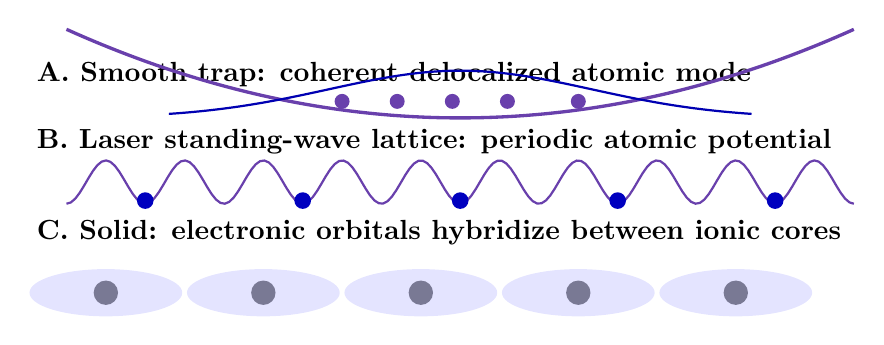
\begin{tikzpicture}[x=1cm,y=1cm,>=Latex]
\node[anchor=west,font=\bfseries] at (0,3.2) {A. Smooth trap: coherent delocalized atomic mode};
\draw[violet,very thick,domain=0.5:10.5,samples=90] plot (\x,{2.65+0.045*(\x-5.5)^2});
\draw[blue!70!black,thick,domain=1.8:9.2,samples=90] plot (\x,{2.65+0.6*exp(-0.18*(\x-5.5)^2)});
\foreach \x in {4,4.7,5.4,6.1,7} \fill[violet] (\x,2.86) circle (2.7pt);
\node[anchor=west,font=\bfseries] at (0,2.35) {B. Laser standing-wave lattice: periodic atomic potential};
\draw[violet,thick,domain=0.5:10.5,samples=180] plot(\x,{1.56+0.55*(sin(180*(\x-0.5)))^2});
\foreach \x in {1.5,3.5,5.5,7.5,9.5} \fill[blue!75!black] (\x,1.60) circle (3pt);
\node[anchor=west,font=\bfseries] at (0,1.2) {C. Solid: electronic orbitals hybridize between ionic cores};
\foreach \x in {1,3,5,7,9} {\fill[black!60] (\x,.43) circle (4.4pt);\fill[blue!35,opacity=.3] (\x,.43) ellipse (.97cm and .3cm);}
\end{tikzpicture}\end{center}
\section{Optical standing waves and atomic light shifts}
Two counter-propagating coherent laser beams generate $E(x,t)=2E_0\cos(kx)\cos(\omega t)$. The intensity varies as $\cos^2(kx)$. For an off-resonant light field the AC Stark shift produces a conservative potential $V(x)\propto I(x)$, with sign determined by the relevant detuning and polarizability. Choosing the origin at an intensity minimum or maximum appropriately, write
\begin{equation}\boxed{V(x)=V_0\sin^2(kx),\qquad k=\frac{2\pi}{\lambda_L},\qquad a=\frac{\pi}{k}=\frac{\lambda_L}{2}.}\end{equation}
The electronic structure mediates the light shift but remains approximately in its prepared internal state: an off-resonant lattice does not require persistent real $5s\to5p$ excitation. Scattering and differential light shifts may nevertheless matter experimentally.
\ex{1: lattice spacing} For $\lambda_L=1064$ nm, $a=532$ nm. A millimeter spans approximately $1.88\times10^3$ sites along one axis. An optical lattice is therefore far more widely spaced than a conventional atomic solid.
\section{The recoil energy and harmonic wells}
The natural energy unit is the single-photon recoil scale
\begin{equation}\boxed{E_R=\frac{\hbar^2k^2}{2M}=\frac{h^2}{2M\lambda_L^2},\qquad M(^{87}\mathrm{Rb})\simeq1.44316\times10^{-25}\;\mathrm{kg}.}\end{equation}
\ex{2: recoil scale at 1064 nm} Substitution gives $E_R/h\simeq2.03$ kHz and $E_R/k_B\simeq97.3$ nK. The optical photon energy is much greater than the motional recoil scale; the two energies must not be conflated.
Near a minimum, $\sin^2(kx)\simeq k^2x^2$, hence $\tfrac12M\omega_{\rm well}^2x^2\simeq V_0k^2x^2$ and
\begin{equation}\boxed{\omega_{\rm well}=\frac{2\sqrt{V_0E_R}}{\hbar}=\frac{2\sqrt{s}E_R}{\hbar},\qquad s=\frac{V_0}{E_R}.}\end{equation}
\ex{3: vibrational level spacing} At $s=16$, $\omega_{\rm well}/(2\pi)=8(E_R/h)\simeq16.2$ kHz. The local harmonic levels are separated by $\hbar\omega_{\rm well}$ when the deep-well harmonic approximation applies.
\section{Bloch bands of a whole atom}
The single-atom Hamiltonian is $h_0=-\hbar^2\nabla^2/(2M)+V_{\rm lat}(\mathbf r)$. For a one-dimensional periodic potential $V(x+a)=V(x)$, Bloch's theorem yields
\begin{equation}\boxed{\psi_{nq}(x)=e^{iqx}u_{nq}(x),\qquad u_{nq}(x+a)=u_{nq}(x).}\end{equation}
These $\psi_{nq}$ are \emph{atomic center-of-mass} states. They should not be identified with the bound valence-electron orbitals of Rb. The quasimomentum $q$ is defined modulo reciprocal lattice vectors $2\pi/a$.
\section{Wannier orbitals and the tight-binding approximation}
For a single isolated band with $N_s$ sites, define a localized Wannier function
\begin{equation}w_j(x)=\frac1{\sqrt{N_s}}\sum_q e^{-iqR_j}\psi_q(x),\qquad R_j=ja.\end{equation}
Expanding the atomic field operator within the lowest band gives $\hat\psi(\mathbf r)\simeq\sum_i w_i(\mathbf r)\hat a_i$. The creation operator $\hat a_i^\dagger$ creates a \emph{whole} atom in a motional Wannier orbital. In a nearest-neighbor one-band approximation, $\epsilon(q)=\epsilon_0-2J\cos(qa)$ in one dimension.
\begin{center}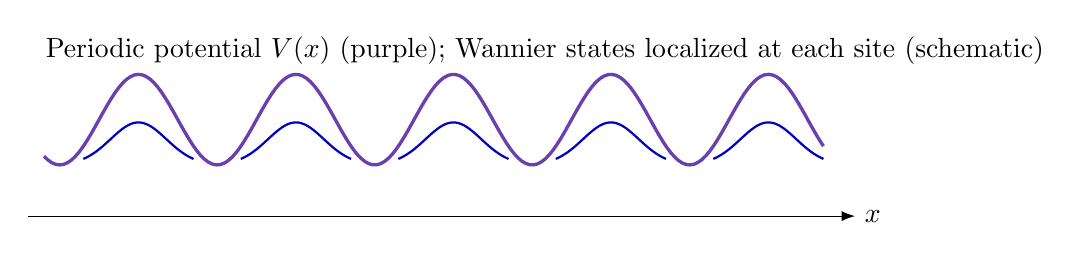
\begin{tikzpicture}[x=1cm,y=1cm,>=Latex]
\draw[->] (0,0)--(10.5,0) node[right]{$x$};
\draw[violet,very thick,domain=0.2:10.1,samples=200] plot (\x,{0.65+1.15*(sin(180*(\x-.4)/2))^2});
\foreach \c in {1.4,3.4,5.4,7.4,9.4} {\draw[blue!75!black,thick,domain=\c-0.7:\c+0.7,samples=36] plot (\x,{.65+.54*exp(-4*(\x-\c)^2)});}
\node[anchor=west] at (.1,2.1) {Periodic potential $V(x)$ (purple); Wannier states localized at each site (schematic)};
\end{tikzpicture}\end{center}
\ex{4: tight-binding bandwidth} For the one-dimensional dispersion $\epsilon(q)=\epsilon_0-2J\cos(qa)$, the minimum and maximum are $\epsilon_0-2J$ and $\epsilon_0+2J$ for $J>0$; the band width is $W=4J$. In a simple cubic nearest-neighbor lattice with $d$ equivalent axes, $W=4dJ$.
For a deep one-dimensional sinusoidal lattice, a useful asymptotic estimate is $J/E_R\approx(4/\sqrt\pi)s^{3/4}e^{-2\sqrt{s}}$. It is not reliable for arbitrarily shallow lattices.
\ex{5: tunneling at $s=16$} Substituting $s=16$ gives $J/E_R\approx(4/\sqrt\pi)8e^{-8}\simeq0.00606$, and hence $J/h\simeq12.3$ Hz. This is an asymptotic estimate rather than an exact diagonalization of a band.
\section{Deriving the Bose--Hubbard model}
With dilute contact interactions $g=4\pi\hbar^2a_s/M$, the continuum many-body Hamiltonian is
\begin{align}\hat H&=\int d^3r\,\hat\psi^\dagger\left[-\frac{\hbar^2\nabla^2}{2M}+V_{\rm lat}(\mathbf r)\right]\hat\psi\\&\quad+\frac g2\int d^3r\,\hat\psi^\dagger\hat\psi^\dagger\hat\psi\hat\psi.\end{align}
After expanding in lowest-band Wannier states and retaining nearest-neighbor kinetic and onsite interaction matrix elements, obtain
\begin{equation}\boxed{\hat H=-J\sum_{\langle i,j\rangle}(\hat a_i^\dagger\hat a_j+\hat a_j^\dagger\hat a_i)+\frac U2\sum_i\hat n_i(\hat n_i-1)+\sum_i(V_i-\mu)\hat n_i.}\end{equation}
Here $U=g\int|w_i(\mathbf r)|^4d^3r$, and $J=-\int w_i^*h_0w_j\,d^3r$ for neighboring sites, with a conventional gauge choice. Additional terms may be required for higher bands, longer-range interactions or density-assisted tunneling. The distinct onsite two-particle energy is $U$, not $2U$, because $U n(n-1)/2=U$ at $n=2$.
\ex{6: onsite interaction energies} A site with $n$ atoms has $E_U(n)=Un(n-1)/2$. For $n=0,1,2,3,4$, the energies are $0,0,U,3U,6U$. The first atom costs no onsite pair-interaction energy; the fourth introduces three additional interacting pairs.
\section{Two competing ground-state regimes}
At weak $U/J$, delocalization and phase coherence dominate, and the superfluid has strong long-range one-body coherence. At strong $U/J$ and integer filling, interaction energy favors a Mott state, approximately $|n_0\rangle_1\otimes\cdots\otimes|n_0\rangle_{N_s}$, with suppressed local number fluctuations and a particle--hole excitation gap. The critical ratio is dimension-, lattice- and filling-dependent; it is not universally $U/J=1$.
\begin{center}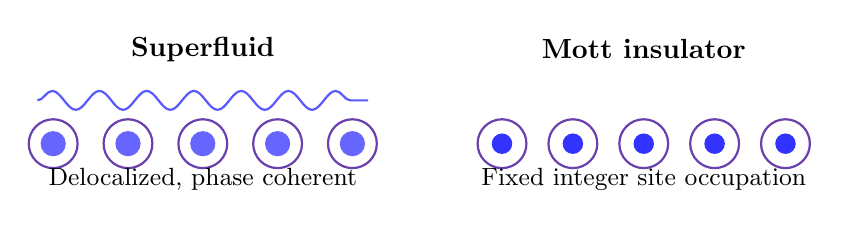
\begin{tikzpicture}[x=1cm,y=1cm]
\node[font=\bfseries] at (2.4,1.65){Superfluid};\node[font=\bfseries] at (8,1.65){Mott insulator};
\foreach \x in {.5,1.45,2.4,3.35,4.3} {\draw[violet,thick] (\x,.45) circle (.31);\fill[blue!60] (\x,.45) circle (.16);}
\draw[blue!65,thick,decorate,decoration={snake,amplitude=1.2mm,segment length=6mm}] (.3,1)--(4.5,1);
\foreach \x in {6.2,7.1,8,8.9,9.8} {\draw[violet,thick] (\x,.45) circle (.31);\fill[blue!80] (\x,.45) circle (.13);}
\node[font=\small] at (2.4,0){Delocalized, phase coherent};\node[font=\small] at (8,0){Fixed integer site occupation};
\end{tikzpicture}\end{center}
\ex{7: number fluctuations} A coherent state with mean $\bar n$ has Poisson statistics $\operatorname{Var}(n)=\bar n$, whereas a site number eigenstate $|n_0\rangle$ has $\operatorname{Var}(n)=0$. The coherent state is an idealized superfluid limit; number-conserving finite lattices need more careful states.
\ex{8: a particle--hole pair in the atomic limit} At unit filling and $J=0$, moving one particle from an occupied site to another creates $(n_i,n_j)=(0,2)$ from $(1,1)$. The energy cost is $U$. For filling $n_0$, changing two sites from $(n_0,n_0)$ to $(n_0-1,n_0+1)$ also costs $U$.
\section{Time-of-flight interference and phase coherence}
After sufficiently long ballistic expansion with negligible interaction effects, the observed momentum distribution approximately samples
\begin{equation}n(\mathbf k)\propto|\widetilde w(\mathbf k)|^2\sum_{i,j}e^{i\mathbf k\cdot(\mathbf R_i-\mathbf R_j)}\langle\hat a_i^\dagger\hat a_j\rangle.\end{equation}
Off-diagonal correlations generate sharp interference peaks; incoherent number states exhibit a broad single-site envelope, although finite-temperature, finite-size and experimental-resolution effects matter. A superfluid--Mott transition in a 3D optical lattice was observed by Greiner et al., \emph{Nature} \textbf{415}, 39--44 (2002).
\ex{9: reciprocal-lattice peak positions} For $a=532$ nm, the reciprocal lattice spacing is $G=2\pi/a\simeq1.18\times10^7$ m$^{-1}$. Far-field interference peaks occur at momenta differing by $\hbar G$; the mapped positions after free flight $t$ differ by $\Delta x=(\hbar G/M)t=(ht)/(Ma)$, under the ballistic approximation.
\ex{10: peak separation after 20 ms} At $t=0.020$ s, $\Delta x=ht/(Ma)\simeq0.173$ mm. This is a convenient imaging scale, distinct from the lattice spacing of 532 nm.
\section{Two-site worked Hamiltonian}
For one atom in two sites, in the basis $|1,0\rangle,|0,1\rangle$, the Hamiltonian is $H=\begin{pmatrix}0&-J\\-J&0\end{pmatrix}$. Its eigenvalues are $-J,+J$ and eigenvectors $(|1,0\rangle\pm|0,1\rangle)/\sqrt2$, with corresponding sign. Starting in $|1,0\rangle$, the probability of finding the atom in the other site after time $t$ is $P_{0,1}(t)=\sin^2(Jt/\hbar)$. The characteristic transfer times are set by $J/\hbar$.
\section{Relation to electronic orbitals and real solids}
A conventional crystal may form overlapping electronic atomic orbitals and electronic Bloch states, e.g. $\psi_{n\mathbf k}^{(e)}(\mathbf r)=e^{i\mathbf k\cdot\mathbf r}u_{n\mathbf k}^{(e)}(\mathbf r)$. An optical lattice also has Bloch and Wannier functions, but its coordinates and particles are \emph{whole neutral atoms}, and its periodic potential is produced by lasers. The formal mathematical structures can resemble each other without implying that the underlying wavefunctions describe the same degrees of freedom. A dilute Rb condensate is not one enormous Rb electron cloud.
\section{Experimental caveats and connections}
The Tiangong picokelvin result concerns an optical dipole-trap Bose condensate and its extremely slow free expansion in microgravity. It should not be represented as a measurement of the superfluid--Mott transition in a standing-wave optical lattice. Optical dipole traps are often smooth; optical lattices are purposely spatially periodic. The long expansion time itself is not evidence of a lattice.
\section{Problems for further study}
\begin{enumerate}[label=\textbf{P\arabic*.}]
\item Derive the first Brillouin zone from $V(x+a)=V(x)$ and locate the degeneracy of free-atom parabolas at the zone boundary.
\item Derive $\omega_{\rm well}$ by Taylor-expanding $V_0\sin^2(kx)$ at a minimum.
\item Evaluate the noninteracting band width of a two-dimensional square lattice with equal $J$ along both directions.
\item Show from the canonical commutation relations that $\hat n(\hat n-1)=\hat a^\dagger\hat a^\dagger\hat a\hat a$.
\item Calculate the onsite interaction energies for $n=0,\ldots,5$ and identify all pair counts.
\item Diagonalize the one-particle two-site Bose--Hubbard Hamiltonian and check oscillation probabilities.
\item Explain why the absolute phase of an isolated number state does not produce a nonzero $\langle\hat a_i\rangle$.
\item Show how a finite interaction-driven Mott gap differs from a conventional single-electron band gap.
\end{enumerate}
\section{References and scope}
\begin{enumerate}
\item I. Bloch, J. Dalibard and W. Zwerger, ``Many-body physics with ultracold gases,'' \emph{Reviews of Modern Physics} \textbf{80}, 885 (2008). DOI: \href{https://doi.org/10.1103/RevModPhys.80.885}{10.1103/RevModPhys.80.885}.
\item M. Greiner et al., ``Quantum phase transition from a superfluid to a Mott insulator in a gas of ultracold atoms,'' \emph{Nature} \textbf{415}, 39--44 (2002). DOI: \href{https://doi.org/10.1038/415039a}{10.1038/415039a}.
\item D. Jaksch et al., ``Cold bosonic atoms in optical lattices,'' \emph{Physical Review Letters} \textbf{81}, 3108 (1998).
\end{enumerate}
\textbf{Editorial scope.} Numerical examples are explicitly modeled scenarios and should not be confused with direct measurements from a particular Tiangong or optical-lattice experiment. The single-band Bose--Hubbard model assumes sufficiently well separated bands, dilute interactions and a suitable filling regime.

\clearpage
\section*{Supplementary Sections to Chapter III: deeper explanations (original chapter preserved)}
\addcontentsline{toc}{section}{Supplementary Sections to Chapter III}
\subsection*{III-A. From the optical AC Stark shift to a lattice potential}
In a far-detuned scalar approximation, an induced dipole $\mathbf p=\alpha(\omega_L)\mathbf E$ produces the time-averaged potential $V_{\rm dip}(\mathbf r)=-\tfrac12\langle\mathbf p\cdot\mathbf E\rangle=-\tfrac14\operatorname{Re}\alpha(\omega_L)E_0^2(\mathbf r)$ for a field whose quoted $E_0$ is its peak amplitude. Two counter-propagating beams generate a standing-wave intensity $\propto\cos^2(kx)$ and therefore a periodic dipole potential. The detuning sign determines whether atoms favor intensity maxima or minima; optical scattering and tensor/vector light shifts can become important outside this simplified model. The laser addresses internal electronic polarizability while generating an external center-of-mass potential.
\subsection*{III-B. A harmonic approximation near one lattice minimum}
For $V(x)=sE_R\sin^2(kx)$ near $x=0$, $\sin(kx)\simeq kx$, so $V\simeq sE_R k^2x^2$. Equating this with $\tfrac12M\omega_{\rm lat}^2x^2$ yields
\begin{equation}\hbar\omega_{\rm lat}=2\sqrt{s}\,E_R.\end{equation}
This predicts local vibrational levels and the approximate width of a lowest-band Wannier state $\ell_{\rm ho}=\sqrt{\hbar/(M\omega_{\rm lat})}=1/(k s^{1/4})$. Increasing the lattice depth $s$ shrinks the onsite wavepacket while suppressing tunneling between adjacent minima.
\begin{example}[Local excitation frequency]
For a 1064-nm Rb-87 lattice with $E_R/h\simeq2.03$ kHz and depth $s=9$, the harmonic spacing is $(\hbar\omega_{\rm lat})/h=2\sqrt9\,E_R/h\simeq12.2$ kHz. This level spacing belongs to whole-atom motion.
\end{example}
\subsection*{III-C. Where the Hubbard approximation fails}
The one-band, nearest-neighbor Bose--Hubbard model assumes the lowest-band Wannier functions dominate, higher-band gaps exceed the relevant interactions and driving frequencies, and the atoms interact primarily through onsite terms. Strong forces, broad Feshbach resonances, density-assisted tunneling, near-resonant light scattering and finite-temperature occupations can invalidate these assumptions. Additional terms include next-neighbor hopping, longer-range interactions, site offsets, and multiband excitations. Thus $U/J$ is powerful but not a complete description of every optical-lattice experiment.
\subsection*{III-D. Electronic crystal versus optical lattice: an operator-level distinction}
For an electronic tight-binding model $c_i^\dagger$ creates an electron in an electronic Wannier orbital centered on an ion site. For an atomic Bose--Hubbard simulator $a_i^\dagger$ creates an entire Rb atom in a center-of-mass Wannier mode defined by light. The mathematical hopping term $-J\sum_{\langle i,j\rangle}(a_i^\dagger a_j+\mathrm{h.c.})$ resembles electronic band theory, but the constituent statistics, interactions, and observables can differ. In particular, atoms are bosons, while electrons are fermions.
\subsection*{III-E. Interference peaks and finite measurement resolution}
A released lattice sample has momentum distribution $n(\mathbf k)\propto|\widetilde w(\mathbf k)|^2\sum_{ij} e^{i\mathbf k\cdot(\mathbf R_i-\mathbf R_j)}\langle a_i^\dagger a_j\rangle$. The Wannier envelope, finite lattice size, inhomogeneous density, imaging resolution, and expansion interactions affect peak height and width. Suppressed peaks do not uniquely prove a perfectly pure Mott state; additional characterization is needed.

\end{document}
